\documentclass{beamer}  

\usetheme{Berlin}
\usetheme{boxes}
\usepackage[spanish]{babel}
\usepackage[T1]{fontenc}
\usepackage[utf8]{inputenc}
\usepackage{graphicx}
\usepackage{tikz}
\usepackage{etex}

\title{Nucleotide String Library}
\author{~Delgado Quesada Juan Jos\'e (B42250)\\
Fallas Pizarro Jose Ariel (B42481)\\
Martinez Garcia David (B34019)
}

\institute[Universidad de Costa Rica] 
{
  Escuela de Ingenier\'ia El\'ectrica\\
  Facultad de Ingenier\'ia \\
  Universidad de Costa Rica}

\date{Proyecto Grupal, II Semestre, 2015 \\
		IE-0217}

\AtBeginSubsection[]
{
  \begin{frame}<beamer>{Outline}
    \tableofcontents[currentsection,currentsubsection]
  \end{frame}
}

\begin{document}

\begin{frame}
  \titlepage
\end{frame}

\begin{frame}
Nucleotidos:
\frametitle{Nucleotide String Library}
\begin{columns}[c]
 \column{.3\textwidth}  
  	\begin{figure}
		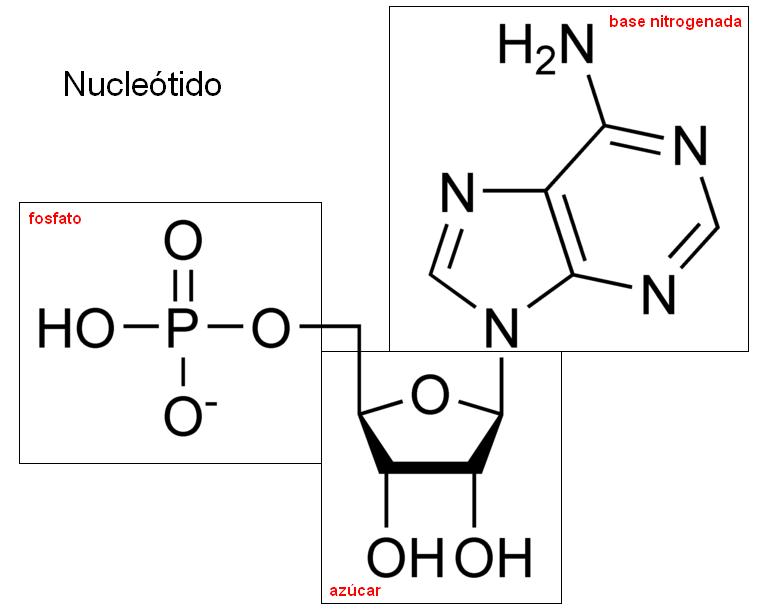
\includegraphics[width=1.7in]{nucleotido.jpg}
	\end{figure}
 \column{.6\textwidth}
 		\begin{figure}
		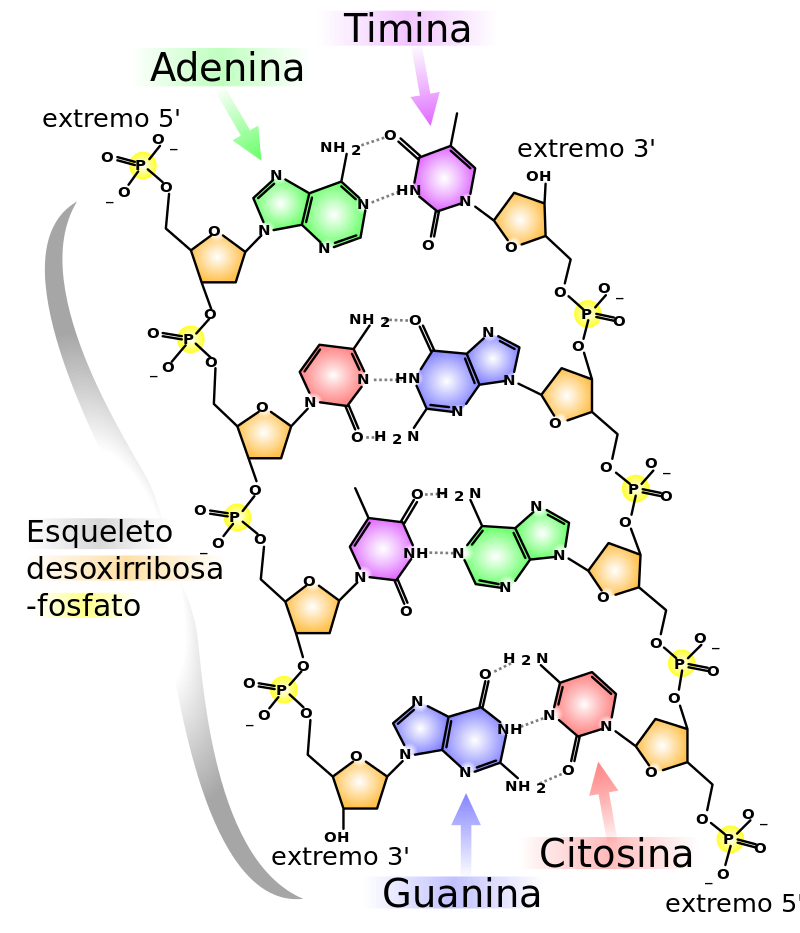
\includegraphics[width=2.0in]{cadena.png}
	\end{figure}
 \end{columns}
\end{frame}

\begin{frame}
\frametitle{Nucleotide String Library}
\textbf{\large{Clase NucleoString :}}
\begin{itemize}
\item{Sumar y Restar}
\item{Comparar}
\end{itemize}
\begin{figure}
		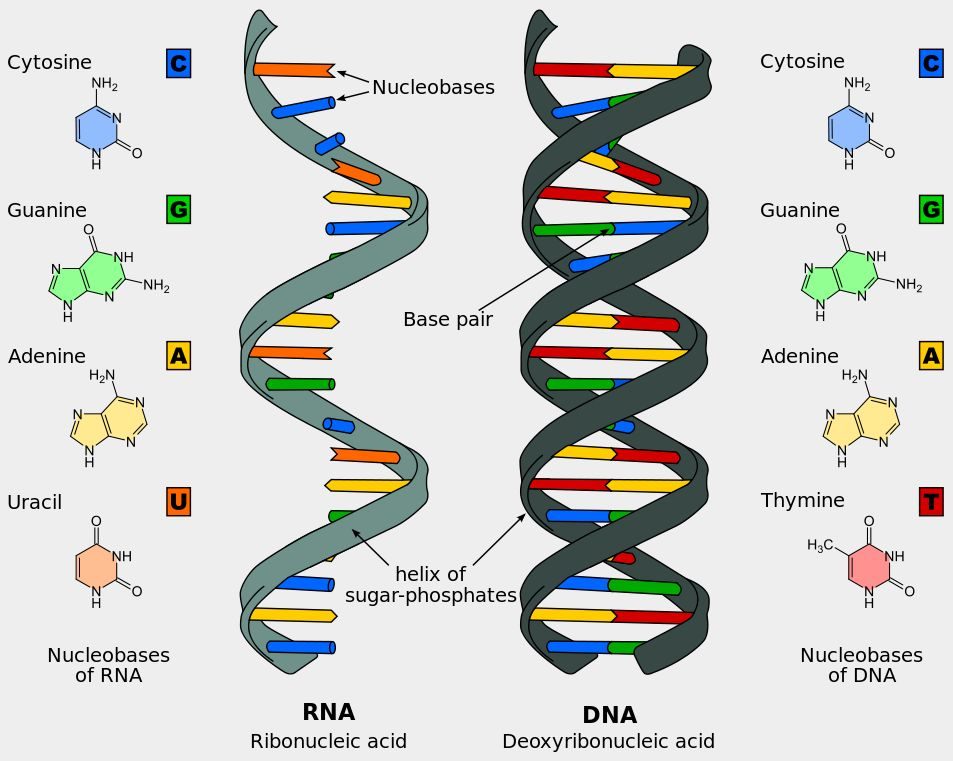
\includegraphics[width=2.5in]{ADN1.jpg}
\end{figure}
\end{frame}

\begin{frame}
\frametitle{Nucleotide String Library}
\textbf{\large{Clase NucleoString :}}
\begin{itemize}
\item{Unir, invertir}
\item{S.complementaria}
\item{Cortar}
\end{itemize}
\begin{figure}
		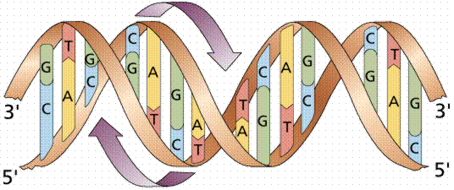
\includegraphics[width=2.5in]{ADN.jpg}
\end{figure}
\end{frame}

\begin{frame}
\frametitle{Nucleotide String Library}
\textbf{\large{Clase Experimento :}}
\begin{itemize}
\item \ Clase compuesta por punteros a muestras
\\
\item \ Nivel más general de muestras. Métodos que trabajen sobre los datos de un muestreo.
\end{itemize}
\end{frame}

\begin{frame}
\frametitle{Nucleotide String Library}
\textbf{\large{Clase NucleoIdent :}}
\begin{itemize}
\item{C.pertencia, Bdominancia}
\item{Es.Desviaci\'on, Imp.Cost}
\item{Grafix}
\end{itemize}
\begin{figure}
		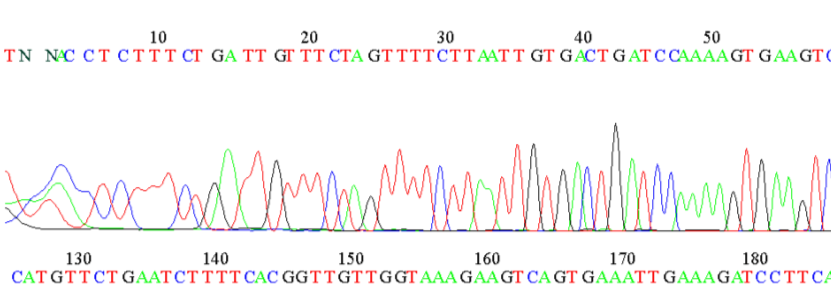
\includegraphics[width=3.7in]{muestra.png}
\end{figure}
\end{frame}

\begin{frame}
\textbf{\large{Clase connections :}} \\
Esta clase es la encargada de administrar las conexiones con la pagina web, para poder postear información, bajar información y datos, entre otras cosas.
\begin{block}{}
\begin{itemize}
\item Se utiliza libcurl, de hecho, Connections hereda de ella
\end{itemize}
\end{block}
\frametitle{Nucleotide String Library}
\end{frame}

\begin{frame}
\textbf{\large{Clase connections :}} \\
Hasta el momento se ha trabajado con la lectura del sourcecode de la pagina.
\begin{block}{}
\begin{itemize}
\item Es posible bajar el sourcecode de la pagina.
\item Se ha comenzado a trabajar con el procesamiento del c\'odigo fuente para accesar la informaci\'on y los datos.
\end{itemize}
\end{block}
\frametitle{Nucleotide String Library}
\end{frame}

\begin{frame}
\frametitle{Nucleotide String Library}
\begin{itemize}
\item{Nucleo.rise, Nucleo.lower }
\item{Ident.Find, Query.Find}
\end{itemize}
\begin{figure}
		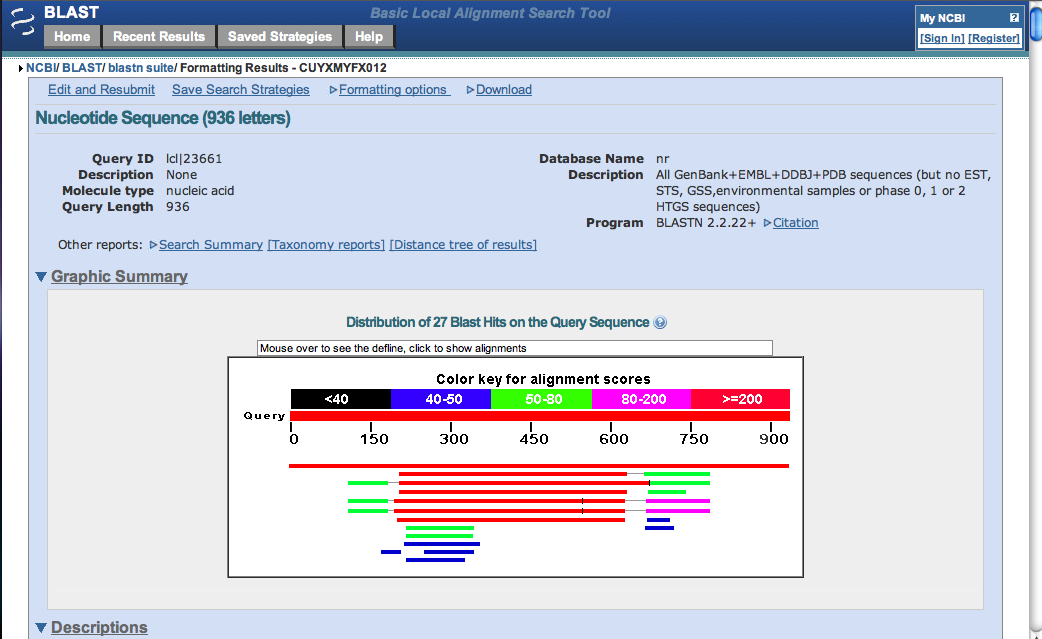
\includegraphics[width=3.2in]{BLAST.png}
\end{figure}
\end{frame}

\begin{frame}
\frametitle{Nucleotide String Library}
\textbf{\large{Centro de Investigaci\'on en Biolog\'ia celular y molecular}}
\begin{figure}
		
\includegraphics[width=1.5in]{CIB.png}
\end{figure}
\end{frame}

\begin{frame}
\frametitle{Nucleotide String Library}
\textbf{\large{Centro de Investigaci\'on en Biolog\'ia celular y molecular}}
\begin{figure}
		
\includegraphics[width=1.5in]{CIB.png}
\end{figure}
\end{frame}

\begin{frame}
\frametitle{Nucleotide String Library}
\textbf{\large{Subclase NucleoARN :}}
\begin{itemize}
\item{An\'alisis de los amino\'cidos }
\end{itemize}
\begin{figure}
		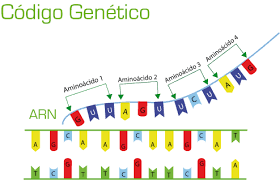
\includegraphics[width=3.2in]{image.png}
\end{figure}
\end{frame}

\begin{frame}
\frametitle{Nucleotide String Library}
\textbf{\large{Subclase NucleoARN :}}
\begin{itemize}
\item{An\'alisis de los amino\'acidos }
\end{itemize}
\begin{figure}
		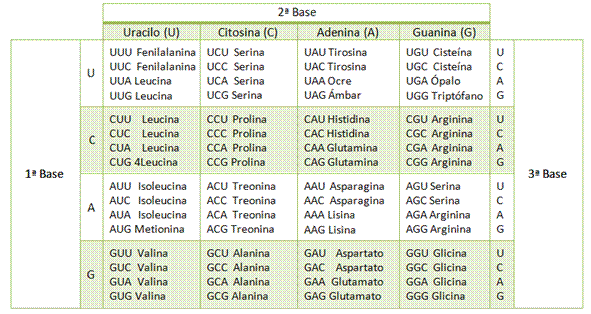
\includegraphics[width=3.6in]{images1.png}
\end{figure}
\end{frame}


\end{document}